One thing to have in mind when it comes to design, is colours. It is difficult to choose which colours to use when designing an interactive system like a webpage. For example, Microsoft use blue in their Windows operating systems as a background colour because blue means calm. Apple uses gray in their products which gives a sense of neutrality. The color blue also gives a sense of neutrality, and suits these products since it caters to a large amount of people, and therefore has to remain neutral. In Figure \ref{Colors} it is shown how the majority of the world reacts when they see different colors. The figure originates from \cite{DEBBook}.

\begin{figure}[htb]
\centering
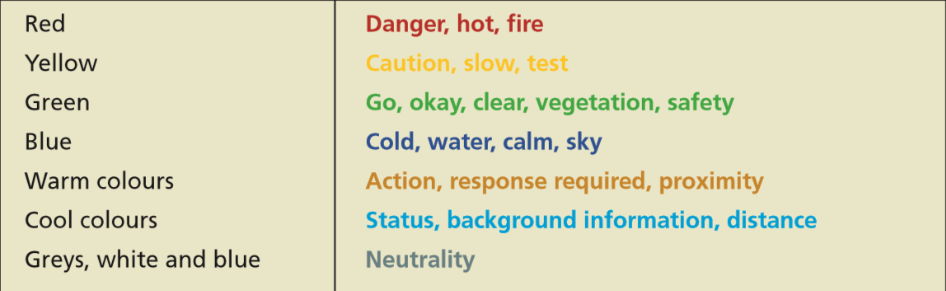
\includegraphics[width=0.8\textwidth]{Images/Colors.png}
\caption{Colors and their interactive meanings \cite{DEBBook}}
\label{Colors}
\end{figure}

In Figure \ref{Login} you can see the general design of the systems login screen, which is also the early version of it. The idea was to keep it simple and smooth with nothing to distract the user from the core features of the system. Since it is a login screen, it is simple and it only has a few buttons and few interactions with the user. Considering how wide the target audience can be for the area of this project, you have to consider colours that cater to various age groups. The colour chosen for our login screen are blue and white, which according to the table expresses calm and neutrality.

\begin{figure}[htb]
\centering
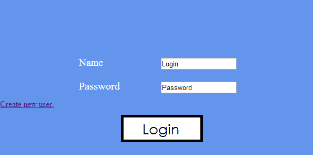
\includegraphics[width=0.6\textwidth]{Images/Login.png}
\caption{Early design of the login screen}
\label{Login}
\end{figure}

When you get past the login screen you will be directed to the front page. On the front page you can access the core features available to the user in the system. The colours from the login screen were also used for the rest of the webpage, to keep it consistent and simple, and to match the target audience. The front page also has a profile image with the username besides it, to indicate that the user is logged in, and several buttons in a global navigation bar to access different features. See Figure \ref{CurrSite} for the early design of the graphical user interface.

\begin{figure}[htb]
\centering
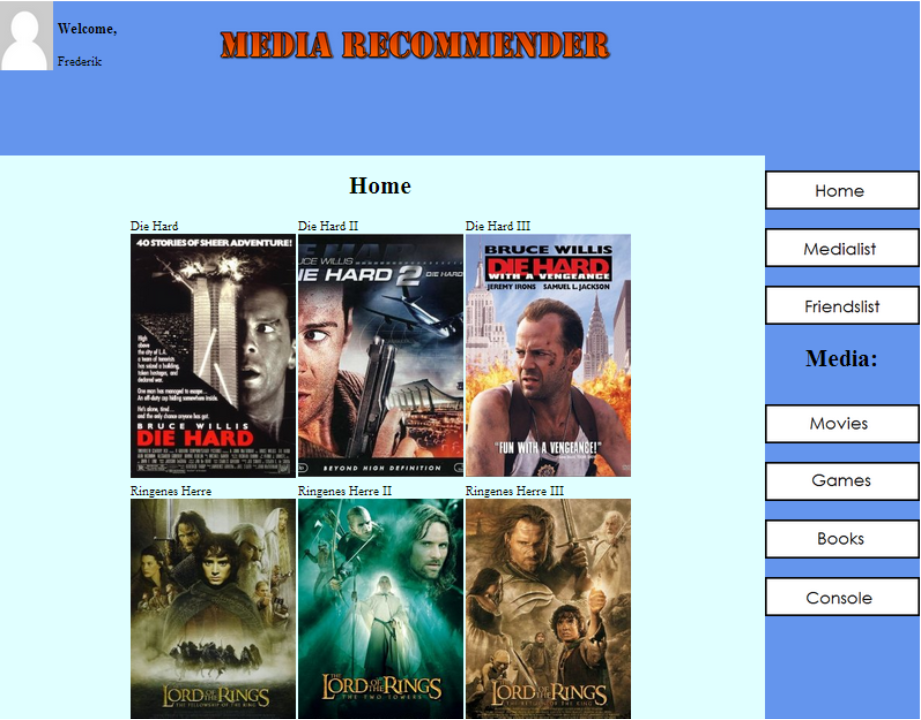
\includegraphics[width=0.8\textwidth]{Images/CurrSite.png}
\caption{Early iteration of the website design}
\label{CurrSite}
\end{figure}


If you look at the prototype of the website, which were made early in the project, it does not deviate much from the early design iteration. See Figure \ref{OldSite}. We have the same elements like the profile picture and username, but have removed the option to insert new media into users' medialist from the search bar that was placed at the top of the website. The new idea is that by simply clicking on the picture, the selected media item is added to the users’ medialist. Also among the removed features is the option to chat with others through the website, which was scraped, together with other ideas for social interaction between users on the website. At this point, the only remaining social feature is the friends list. 

Instead of a home button with a traditional house icon in the lower right corner, it was moved up to take a more central placement at the top of the buttons. In this iteration of the design process, the home page was planned to be one of the central pages of the website, being the page users use to add media to their medialists. The more central placement is to provide added convenience to the user. The home page is also planned to offer media searching and media rating features.

The navigation bar on the right side has also taken a more important role and acts as a gateway for the user to the systems features. Instead of just containing pages for looking through each media type available to the system, the navigation now also holds buttons to the now important home page, and the users’ medialist.
	
\begin{figure}[htb]
\centering
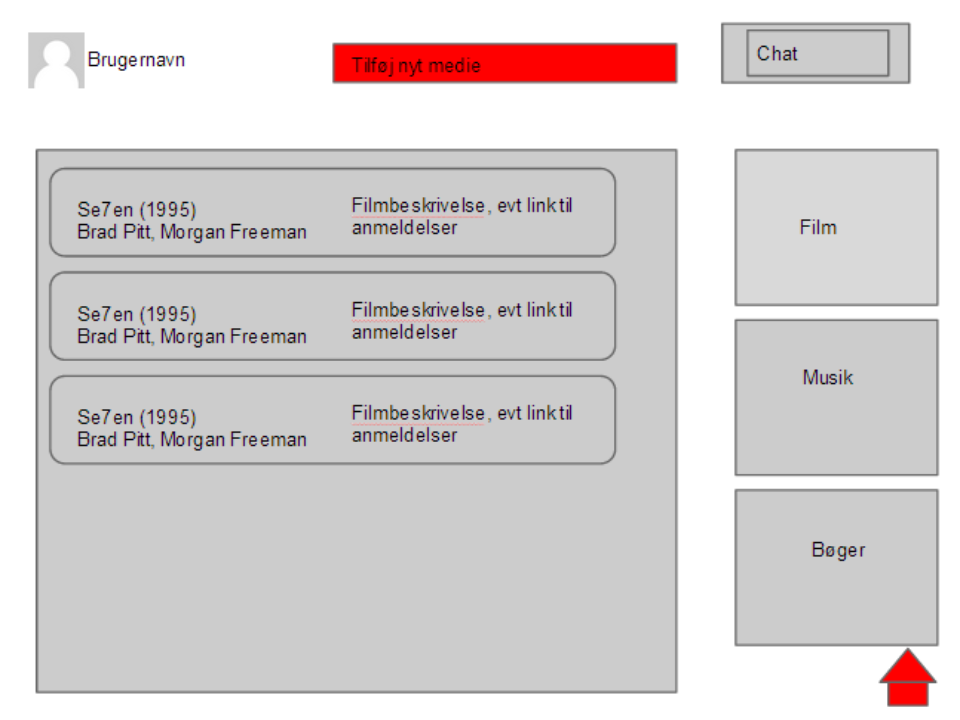
\includegraphics[width=0.8\textwidth]{Images/OldSite.png}
\caption{Early prototype of the website design}
\label{OldSite}
\end{figure}